\chapter{How do I...?}
This chapter isn't part of my thesis, rather it's an aide-memoir so I can work out how do I do various things such as provide an attractively formatted code snippet.

\section{Source code}
Use minted, \textit{e.g.} Listing \ref{examplelisting:build_gradle_for_sentry}, and for more examples see \url{https://www.overleaf.com/learn/latex/Code_Highlighting_with_minted}.

\begin{listing}
\begin{minted}{groovy}
dependencies {
    implementation 'io.sentry:sentry-android:6.0.0'
}
\end{minted}
\caption{Example: Install Sentry \texttt{build.gradle} to an Android app's codebase\\source: \href{https://docs.sentry.io/platforms/android/}{Android Sentry Documentation}}
\label{examplelisting:build_gradle_for_sentry}
\end{listing}

\section{References including internal cross-references}
A locally defined latex command \texttt{\\secref{}} combines \\autoref\{\#1\} and \\nameref\{\#1\}. 
Usage example: \texttt{\\secref\{section:my\}}, from \url{https://stackoverflow.com/a/30844515/340175}.

\section{Side-by-side figures}
Use minipages. For example:

\begin{figure}[htbp!]
\centering
\begin{minipage}{.45\textwidth}
  \centering
  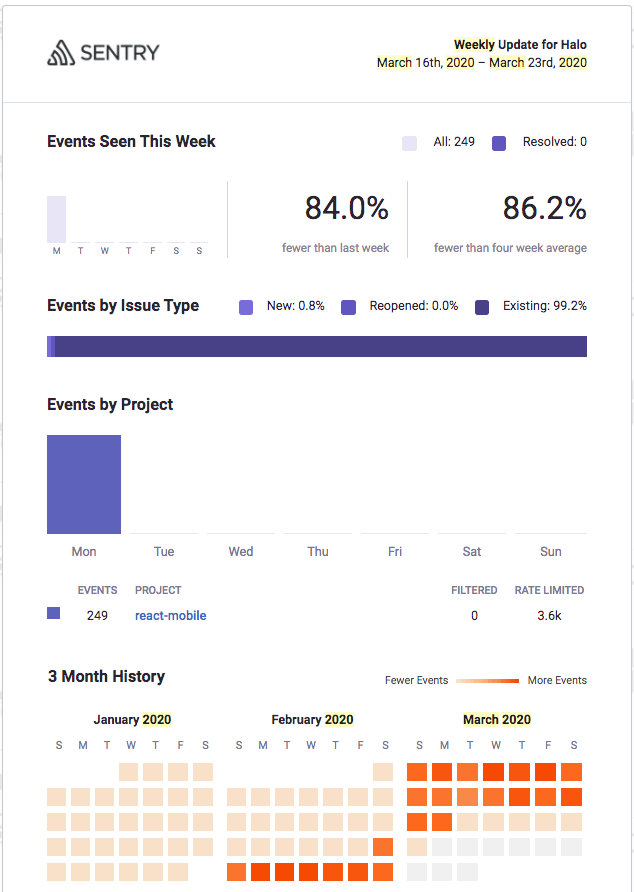
\includegraphics[width=\textwidth]{images/localhalo/sentry-weekly-report-16-mar-2020.png}
  \captionof*{figure}{\nth{16} -~\nth{22} March 2020}
  \label{fig:localhalo-sentry-weekly-report-16-mar-2020}
\end{minipage}\hfill%
\begin{minipage}{.45\textwidth}
  \centering
  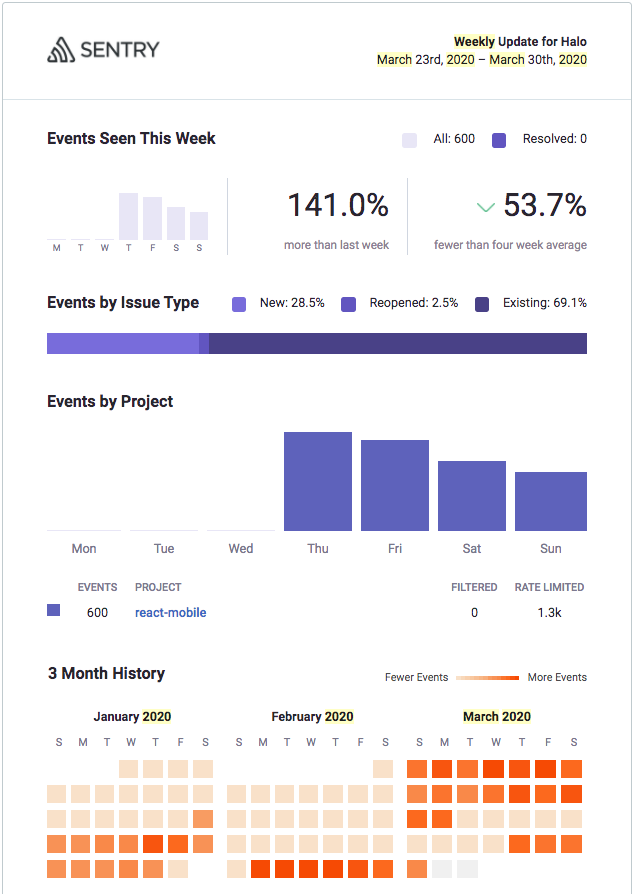
\includegraphics[width=\textwidth]{images/localhalo/sentry-weekly-report-23-mar-2020.png}
  \captionof*{figure}{\nth{23} -~\nth{29} March 2020}
  \label{fig:localhalo-sentry-weekly-report-23-mar-2020}
\end{minipage}
    \caption{Missing data reported in Sentry, in March 2020}
    \label{fig:sentry-missing-data-march-2020}
\end{figure}

\section{Punctuation}

For ellipses (\ldots) use \texttt{\\ldots}.